\documentclass[tikz,border=6pt]{standalone}
\usepackage{amsmath}
\begin{document}
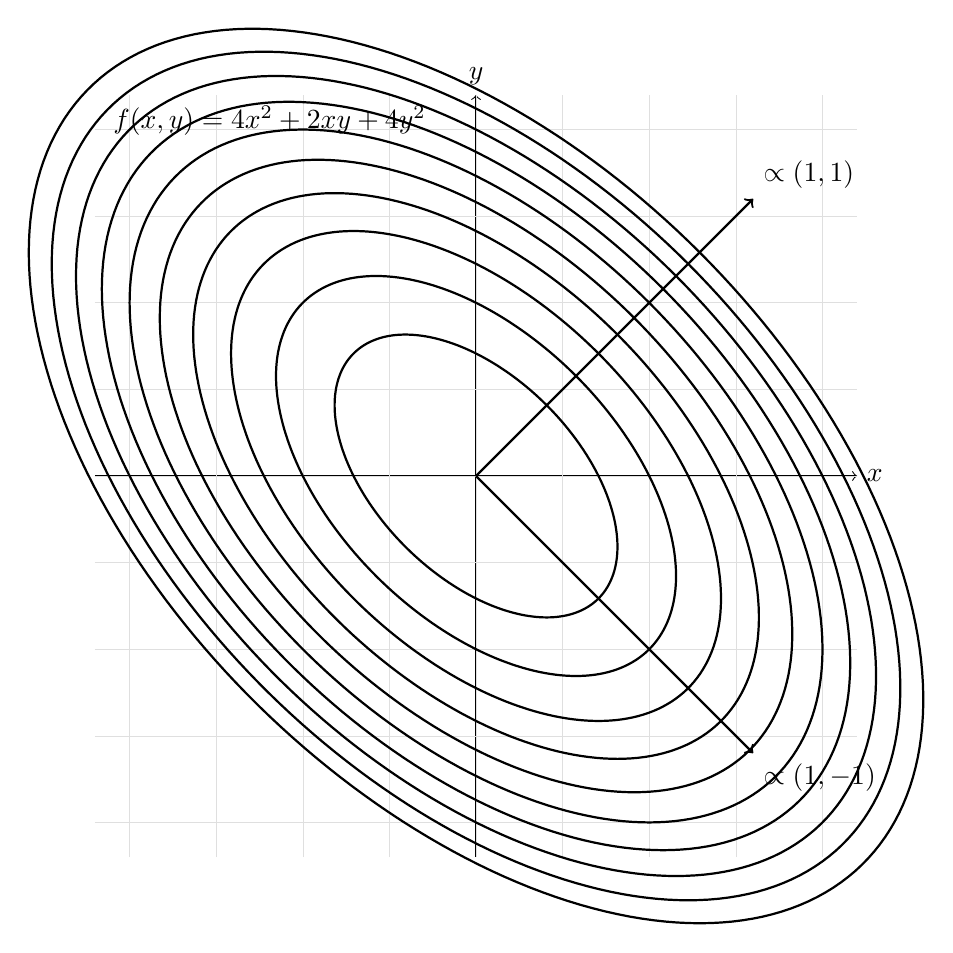
\begin{tikzpicture}[scale=2.2]

% axes
\draw[->] (-2.2,0) -- (2.2,0) node[right] {$x$};
\draw[->] (0,-2.2) -- (0,2.2) node[above] {$y$};

% light grid (optional)
\draw[step=0.5, very thin, gray!25] (-2.2,-2.2) grid (2.2,2.2);

% principal directions (optional)
\draw[->, thick] (0,0) -- (1.6,1.6) node[above right] {$\propto(1,1)$};
\draw[->, thick] (0,0) -- (1.6,-1.6) node[below right] {$\propto(1,-1)$};

% Draw level sets f(x,y)=c for selected c values
% You can edit the list {2,4,6,...} as you like.
\foreach \c in {2,4,6,8,10,12,14,16,18,20}{

  % semi-axes in (u,v)-coordinates for 6u^2 + 2v^2 = c
  \pgfmathsetmacro{\au}{sqrt(\c/6)} % amplitude for u
  \pgfmathsetmacro{\av}{sqrt(\c/2)} % amplitude for v

  % parametric plot: t in degrees (0..360)
  \draw[thick]
    plot[domain=0:360, samples=220, variable=\t]
    (
      { ( (\au*cos(\t)) + (\av*sin(\t)) ) / sqrt(2) },
      { ( (\au*cos(\t)) - (\av*sin(\t)) ) / sqrt(2) }
    );
}

\node[anchor=west] at (-2.15,2.05) {$f(x,y)=4x^2+2xy+4y^2$};

\end{tikzpicture}
\end{document}

